

\chapter{Conclusions and Future Directions}
\label{cha:conclusions_future_directions}
This chapter synthesizes the insights gleaned from the comprehensive benchmarking of non-blocking IO processing algorithms, as detailed in the preceding chapters. Our investigation spanned various strategies and implementations, culminating in a nuanced understanding of the relative performance and characteristics of different approaches across .NET, Java, and other programming environments. Here, we consolidate these findings, reflecting on their broader implications within the field of asynchronous programming. Furthermore, we outline potential avenues for future research that emerge from our study, paving the way for continued exploration and innovation in this domain.



% Detailed Analysis and Comparison of Results
\section{Detailed Analysis and Comparison of Results}
This section embarks on a meticulous analysis of the benchmarking results obtained from our comprehensive study of asynchronous IO processing algorithms, specifically focusing on the implementations in .NET, Java, and JavaScript environments. Our exploration into these diverse programming landscapes has been guided by a keen interest in understanding how different asynchronous IO tools and pipeline strategies perform under varying conditions and requirements.

The subsequent subsections will dissect and compare the performance of each environment, offering a granular view of their capabilities and limitations in handling the two main algorithms we have focused on: Finding the largest word in a set of files, and the Grouping of words based on their sizes. These algorithms, implemented across .NET, Java, and JavaScript, provide a rich ground for comparison, revealing insights into the nuances of each programming paradigm.



\section{.NET Benchmarking}
\label{sec:dotnet_implementation}

In this subsection, we focus on the benchmark using different strategies in .NET programming environment.



\subsection{Find biggest word algorithm results}
\label{subsubsec:biggest_word_results_cs}

For the find biggest word algorithm, used i .NET implementations are the following strategies:

\begin{itemize}
    \item \textbf{Baseline}: This strategy serves as the basic approach for finding the biggest word and acts as a baseline for comparison.
    \item \textbf{Asynchronous Baseline }: This strategy uses a single asynchronous task to find the biggest word.
    \item \textbf{Parallel }: An approach that makes the use of parallelization.
    \item \textbf{Asynchronous Enumerables}: This approach uses asynchronous programming with enumerable collections.
    \item \textbf{RxNet }: This strategy uses the Reactive Extensions (Rx) library with asynchronous file reading operations.
\end{itemize}


In the following graphic, we have the results in seconds for each strategie:

\begin{figure}[H]
    \centering
    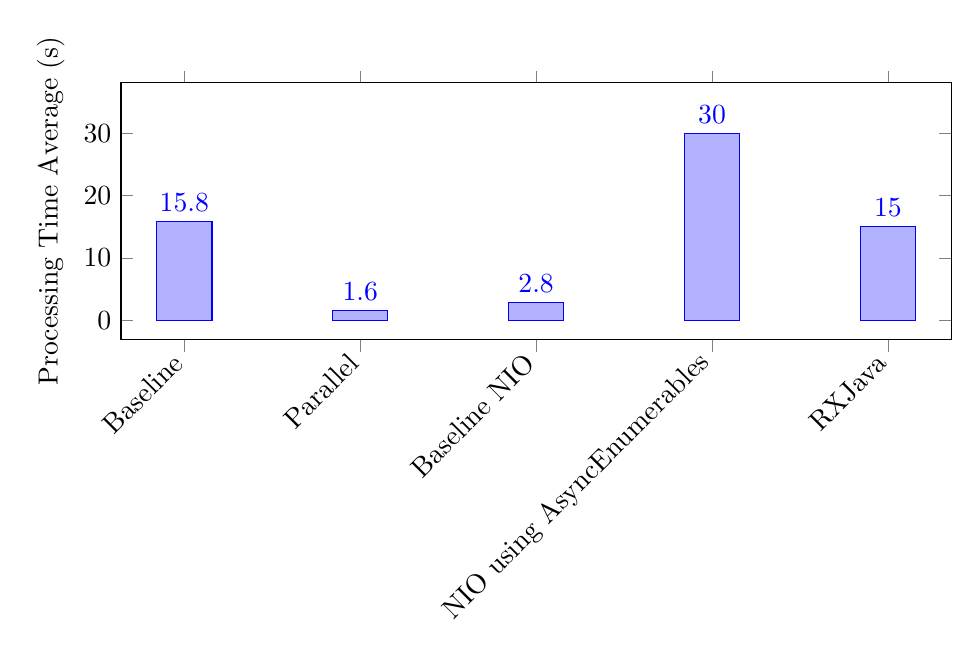
\begin{tikzpicture}
    \begin{axis}[
        ybar=2*\pgflinewidth,
        width=1.0\textwidth,
        height=0.4\textwidth,
        bar width=20pt,
        enlargelimits=0.09,
        legend style={at={(0.5,-0.2)}, anchor=north, legend columns=-1},
        ylabel={Processing Time Average (s)},
        symbolic x coords={Baseline, Parallel, Baseline NIO, NIO using AsyncEnumerables, RXJava},
        xtick=data,
        xticklabel style={rotate=45, anchor=east},
        nodes near coords,
        nodes near coords align={vertical},
        ymin=0, ymax=35,
        ]
    \addplot coordinates {(Baseline, 15.8) (Parallel, 1.6) (Baseline NIO, 2.8) (NIO using AsyncEnumerables, 30) (RXJava, 15)};
    \end{axis}
    \end{tikzpicture}
    \caption{Processing times for different strategies for "Find the biggest word".}
    \label{fig:biggest_word_results_cs_2}
\end{figure}


As we can see from these results, it is evident that the algorithm for "Finding the largest word" in a large file dataset performs worse with blocking IO solutions compared to non-blocking approaches. Furthermore, when considering the various solutions, it becomes apparent that the performance deteriorates as the API complexity increases. An exception to this trend is that, despite leveraging non-blocking IO, AsyncEnumerable exhibits the poorest overall performance.

\clearpage


\subsection{Group Word Results}
\label{subsubsec:group_word_processing_times_cs}

In this subsection, we concentrate on the task of grouping words from a file using different strategies. The strategies that we evaluate here include:

\begin{itemize}
    \item \textbf{Baseline}: This strategy serves as the basic approach for word grouping and acts as a baseline for comparison.
    \item \textbf{Linq}: Like in the find word algorithm, this strategy uses Language Integrated Query (LINQ) in a synchronous manner.
    \item \textbf{AsyncEnumerable}: This strategy uses .NET async enumerables to process the asynchronous data .
    \item \textbf{RxNet}: Here, the Reactive Extensions (Rx) library is used to handle data sequences asynchronously and event-based.
\end{itemize}


%\begin{table}[H]
%    \centering
%    \resizebox{\textwidth}{!}{%
%    \begin{tabular}{|l|c|}
%    \hline
%    \textbf{Strategy} & \textbf{Processing Time Average (s)} \\ \hline
%    Baseline Blocking IO & 26 \\ \hline
%    Linq & 22 \\ \hline
%    Async Enumerable & 30 \\ \hline
%    Rx Net & 22 \\ \hline
%    \end{tabular}%
%    }
%    \caption{Processing times for different strategies for "Count Words".}
%    \label{tab:group_word_processing_times_cs}
%\end{table}

\begin{figure}[H]
    \raggedright
    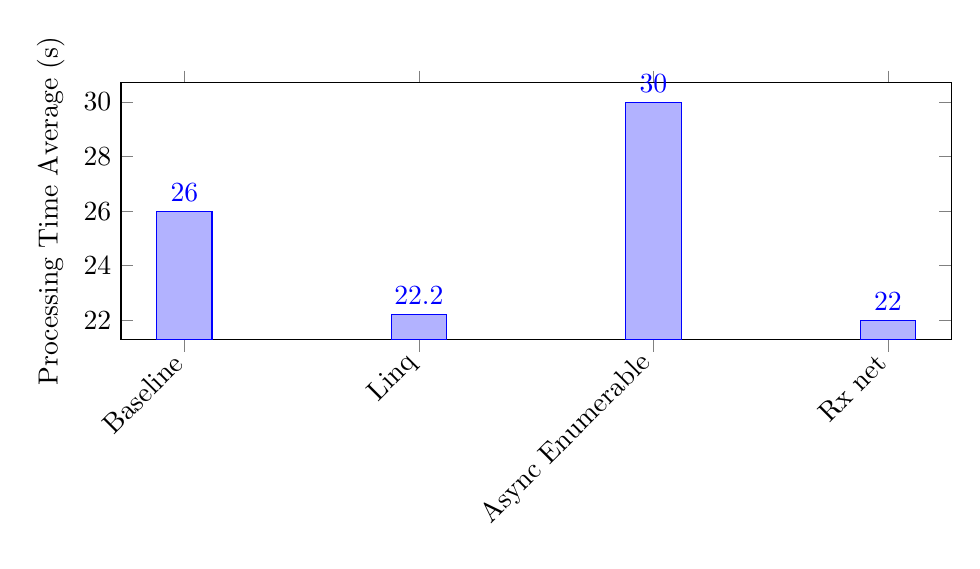
\begin{tikzpicture}
    \begin{axis}[
        ybar=2*\pgflinewidth,
        width=1.0\textwidth,
        height=0.4\textwidth,
        bar width=20pt,
        enlargelimits=0.09,
        legend style={at={(0.5,-0.2)}, anchor=north, legend columns=-1},
        ylabel={Processing Time Average (s)},
        symbolic x coords={Baseline, Linq, Async Enumerable, Rx net},
        xtick=data,
        xticklabel style={rotate=45,anchor=east},
        nodes near coords,
        nodes near coords align={vertical},
        ]
    \addplot coordinates {(Baseline, 26.0) (Linq, 22.2) (Async Enumerable, 30) (Rx net, 22.0)};
    \end{axis}
    \end{tikzpicture}
    \caption{Processing times for different strategies for "Count Words".}
    \label{fig:group_word_processing_times_cs}
\end{figure}

In the case of memory-intensive algorithms like "Group words," which heavily rely on dictionaries, for example, pipeline libraries outperform baseline approaches. However, whether one uses blocking or non-blocking IO operations becomes irrelevant in such scenarios, as memory-intensive operations overshadow any potential gains from using non-blocking IO operations.

\clearpage

\section{Java/Kotlin Benchmarking}
\label{sec:java_implementation}

In this section, we explore and assess diverse strategies applied in Java and Kotlin to process files, and we scrutinize their performances solving the "Find Word" an "Group Word algorithms"


\subsection{Biggest Word Results}
\label{subsubsec:biggest_word_results}

The strategies used in JAVA are:

\begin{itemize}
    \item \textbf{Baseline}: This strategy illustrates a basic non-blocking I/O operation, serving as a comparison baseline.
    \item \textbf{Flux}: These strategies leverage the Reactor Flux model from Java's Project Reactor library. The former follows a standard non-concurrent processing model, while the latter introduces parallelization for improved performance.
    \item \textbf{RXJava}: This strategy employ the RXJava library. They replace the Reactor Flux with Observables, with the distinction being made between non-concurrent and concurrent processing.
    \item \textbf{Streams and parallelization}: Implementation of three strategies that use Java's Streams API and explore handling of blocking operations under three different conditions: standard usage, raw multithreading using threadpools and using parallel method in the streams API.
    
\end{itemize}


In the following graphic, we have the results in seconds for each strategy:

    \begin{figure}[H]
        \raggedright
        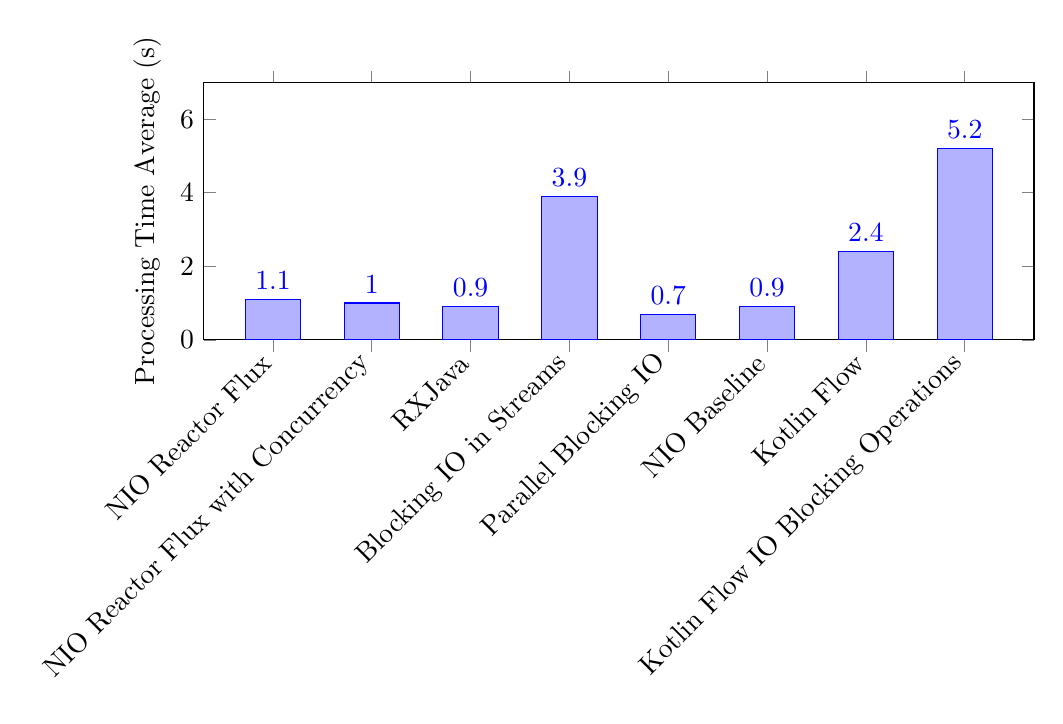
\begin{tikzpicture}
        \begin{axis}[
            ybar=2*\pgflinewidth,
            width=1.0\textwidth,
            height=0.4\textwidth,
            bar width=20pt,
            legend style={at={(0.5,-0.2)}, anchor=north, legend columns=-1},
            ylabel={Processing Time Average (s)},
            symbolic x coords={NIO Reactor Flux, NIO Reactor Flux with Concurrency, RXJava, Blocking IO in Streams, Parallel Blocking IO,  NIO Baseline, Kotlin Flow,  Kotlin Flow IO Blocking Operations},
            xtick=data,
            xticklabel style={rotate=45,anchor=east},
            nodes near coords,
            nodes near coords align={vertical},
            ymin=0, ymax=7,
            ]
        \addplot coordinates {(NIO Reactor Flux, 1.1) (NIO Reactor Flux with Concurrency, 1.0) (RXJava, 0.9)  (Blocking IO in Streams, 3.9) (Parallel Blocking IO, 0.7) (NIO Baseline, 0.9) (Kotlin Flow, 2.4) (Kotlin Flow IO Blocking Operations, 5.2)};
        \end{axis}
        \end{tikzpicture}
        \caption{Processing times for different Java/Kotlin strategies for "Biggest Word".}
        \label{fig:biggest_word_processing_times}
    \end{figure}
    

    \clearpage

    \subsection{Group Word Results}
    \label{subsubsec:group_word_results}
    
   The strategies discussed here include:

    \begin{itemize}
        \item \textbf{Baseline}: This strategy serves as a baseline for comparison. It illustrates a basic non-blocking I/O operation without the use of any high-level constructs like Reactor Flux or Observable.
        \item \textbf{RXJava}: This strategy employs the RXJava library, popular for building asynchronous and event-driven applications.
        \item \textbf{Flux}: This strategy leverages the Reactor Flux model available in Java's Project Reactor library, providing an efficient approach to handling asynchronous data sequences.
        \item \textbf{Parallelization}: This strategy uses Java's Streams API and explores handling of blocking operations with the help of threadpools.
        \item \textbf{Streams}: Similar to the previous strategy, this one uses Java's Streams API, but handles blocking operations within streams.
        \item \textbf{Flow (Kotlin)}: This strategy utilizes Kotlin's Coroutines and Flow API, which are particularly well-suited for handling multiple values that are emitted sequentially.
    \end{itemize}

    In the following table and graphic, we have the results in seconds for each strategy:

    \begin{figure}[H]
        \centering
        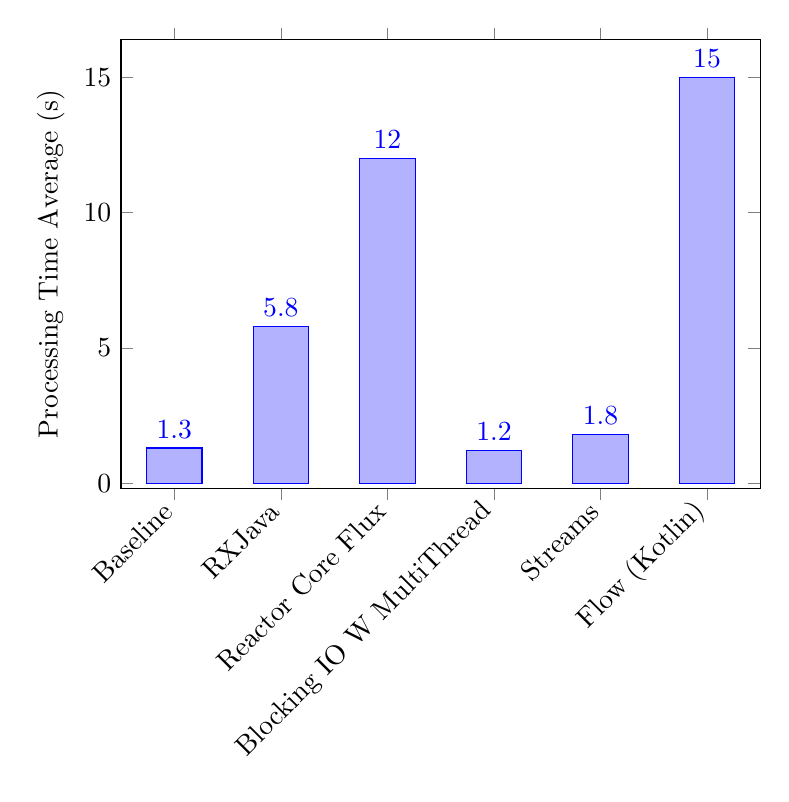
\begin{tikzpicture}
        \begin{axis}[
            ybar=2*\pgflinewidth,
            width=0.8\textwidth,
            height=0.6\textwidth,
            bar width=20pt,
            legend style={at={(0.5,-0.2)}, anchor=north, legend columns=-1},
            ylabel={Processing Time Average (s)},
            symbolic x coords={Baseline, RXJava, Reactor Core Flux, Blocking IO W MultiThread, Streams, Flow (Kotlin)},
            xtick=data,
            xticklabel style={rotate=45,anchor=east},
            nodes near coords,
            nodes near coords align={vertical},
            ]
            \addplot coordinates { (Baseline, 1.3) (RXJava, 5.8) (Reactor Core Flux, 12.0) (Blocking IO W MultiThread, 1.2) (Streams, 1.8) (Flow (Kotlin), 15.0)};
        \end{axis}
        \end{tikzpicture}
        \caption{Processing times for different Java/Kotlin strategies for "Group Words".}
        \label{fig:processing_times}
    \end{figure}
    

    \clearpage
... 
% Here you conclude the entire chapter by summarizing your findings and interpretations.


\section{JavaScript Benchmarking}
\label{sec:js_implementation}


\subsection{Finding the Biggest Word}
\label{subsec:biggest_word_js}

Here, we investigate the following three strategies:

\begin{itemize}
    \item \textbf{Baseline for await..of without pipeline}: This strategy serves as the basic JavaScript approach for finding the biggest word, acting as a baseline for comparison.
    \item \textbf{Baseline for await..of with pipeline}: This strategy uses JavaScript streams, which provide a way to handle reading/writing files, network communications, or any kind of end-to-end information exchange in an efficient manner.
    \item \textbf{RxJS}: This strategy leverages the Reactive Extensions for JavaScript (RxJS) library, which offers a set of methods for dealing with asynchronous data sequences in an effective way.
\end{itemize}


In the following graphic, we have the results in seconds for each strategy:


\begin{figure}[H]
    \raggedright
    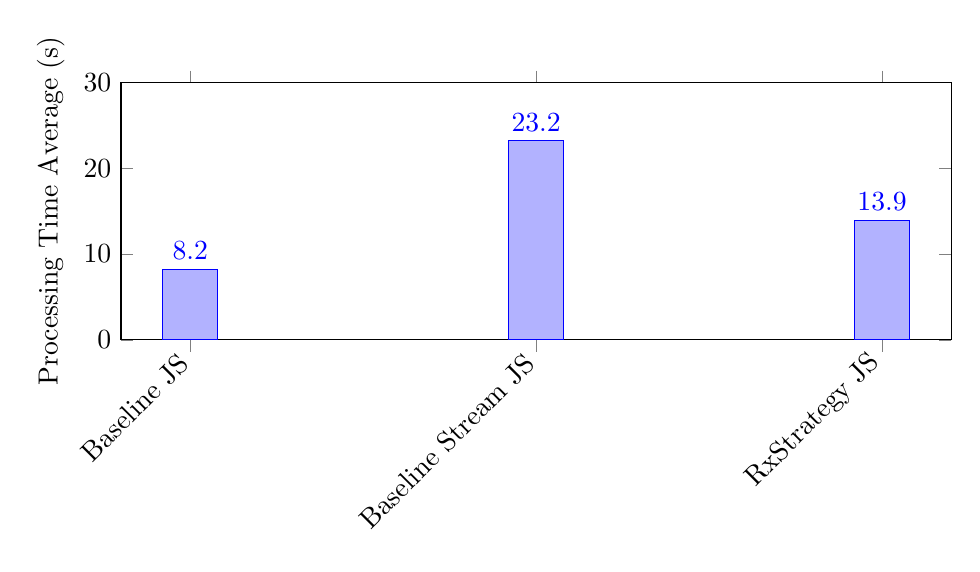
\begin{tikzpicture}
    \begin{axis}[
        ybar=2*\pgflinewidth,
        width=1.0\textwidth,
        height=0.4\textwidth,
        bar width=20pt,
        legend style={at={(0.5,-0.2)}, anchor=north, legend columns=-1},
        ylabel={Processing Time Average (s)},
        symbolic x coords={Baseline JS, Baseline Stream JS, RxStrategy JS},
        xtick=data,
        xticklabel style={rotate=45,anchor=east},
        nodes near coords,
        nodes near coords align={vertical},
        ymin=0, ymax=30,
        ]
    \addplot coordinates {(Baseline JS, 8.2) (Baseline Stream JS, 23.2) (RxStrategy JS, 13.9)};
    \end{axis}
    \end{tikzpicture}
    \caption{Processing times for different JavaScript strategies for "Biggest Word" Graphic}
    \label{fig:biggest_word_processing_times_js}
\end{figure}

As we can see in this javascript implementation, the performance for find biggest word algorithm of the baseline behaves as expected, having the best performance among its alternatives. On the other side, the algorithm implemented using RXJS library behaves slightly better than the alternative that makes use of JS streams API.


\clearpage



\subsection{Grouping Words}
\label{subsec:grouping_words_js}

In this subsection, we evaluate the following strategies for grouping words:

\begin{itemize}
    \item \textbf{Baseline JS}: This strategy serves as the basic JavaScript approach for grouping words, acting as a baseline for comparison.
    \item \textbf{Baseline Stream JS}: This strategy uses JavaScript streams, which provide a way to handle reading/writing files, network communications, or any kind of end-to-end information exchange in an efficient manner.
    \item \textbf{RxStrategy JS}: This strategy leverages the Reactive Extensions for JavaScript (RxJS) library, which offers a set of methods for dealing with asynchronous data sequences in an effective way.
\end{itemize}

In the following graphic, we present the results in seconds for each strategy:


\begin{figure}[H]
    \centering
    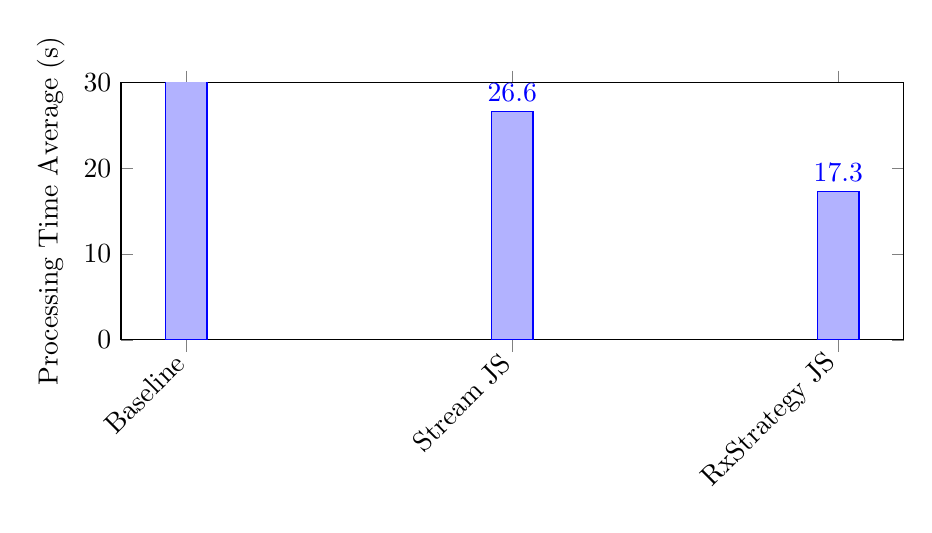
\begin{tikzpicture}
    \begin{axis}[
        ybar=2*\pgflinewidth,
        width=0.95\textwidth,
        height=0.4\textwidth,
        bar width=15pt, % Reduced bar width
        legend style={at={(0.5,-0.2)}, anchor=north, legend columns=-1},
        ylabel={Processing Time Average (s)},
        symbolic x coords={Baseline, Stream JS, RxStrategy JS},
        xtick=data,
        xticklabel style={rotate=45, anchor=east},
        nodes near coords,
        nodes near coords align={vertical},
        ymin=0, ymax=30,
        ]
    \addplot coordinates {(Baseline, 30.1) (Stream JS, 26.6) (RxStrategy JS, 17.3)};
    \end{axis}
    \end{tikzpicture}
    \caption{Processing times for different JavaScript strategies for "Grouping Words" Graphic}
    \label{fig:grouping_words_processing_times_js}
\end{figure}



In this case, the performance of the algorithms change radically from what we saw in the "Find the biggest word" algorithm. In this case, the baseline haves the worst performance among the three strategies, while the RxStrategy haves the best. 
One explanation for these results is that the pipeline instructions of the pipeline instructions are optimized while the baseline is not. 

% Main Conclusions
\section{Main Conclusions}

% Future Work and Recommendations
\section{Future Work and Recommendations}
\subsection{Suggestions for Future Studies}

% Final Thoughts
\section{Final Thoughts}
\subsection{Personal Reflections}
\subsection{Closing Remarks}

% References (if not included at the end of the thesis)
\section*{References}



\end{document}